\documentclass{amsart}
\usepackage[utf8]{inputenc}
\usepackage{tikz}
\usepackage{cite}

\title{Independent Study Group Report}
\author{Arden Rasmussen, Sean Richardson, Adriana Rogers }
\date{Spring 2019}

\begin{document}

\maketitle

\section{Introduction}
% ADRIANA
In our independent study, we aimed to study the mathematical foundations of
neural networks, and other machine learning techniques. We began by following
Stanford's lecture videos from their course, ``CS231n: Convolutional Neural
Networks for Visual Recognition'' \cite{stanford}. This course provided a
foundation for neural networks and convolution, from which we continued our
studies. We also used Goodfellow's book, ``Deep Learning''
\cite{Goodfellow-et-al-2016}.

We quickly realized that analogies to biological neural networks and the brain,
which seem to be unavoidable in many cursory instruction on neural networks,
are misleading. They give rise to the mischaracterization of neural networks as
black boxes. Rather, neural networks ``learn'' by optimizing for some loss
function. At the heart of this method, as we will describe below, are
techniques that we find from linear algebra and  calculus.

Another grievance we had with our study of neural networks, besides the
biological interpretation, was the arbitrary selection of hyper-parameters.
Most importantly, parameters such as the step size of gradient descent and the
learning rate, which we will describe below, are typically set using
guess-and-check, or cross-validation. To ease these frustrations, we began
studying genetic algorithms, as a way to search through the space of possible
hyperparameters to be used to train a neural network to play the game snake.

This report will begin in Section \ref{optimization} by framing our studies as
an optimization problem, giving a general background to optimization. Next, in
Section \ref{neural_networks}, we will give an overview of the architecture of
neural networks, propagation, and convolutional layers for image
classification. In Section \ref{section_genetic}, we will outline the process
of a genetic algorithm to solve optimization problems. Finally, in Section
\ref{section_snake}, we will explain how we used these concepts to train a
neural network to play the game snake.

\section{Optimization} \label{optimization}
% SEAN
%this is a math problem, and these are the CS ways to solve it.

\section{Neural Networks} \label{neural_networks}
%ADRIANA + ARDEN

\subsection{Architecture}\label{sub:architecture}

The structure of a neural network can be broken down into smaller building
blocks. Every network is a connection of layers. Each layer has a different
type, and does a different action. Some of the common layer types are described
here.
\begin{description}
  \item[Input] The input layer takes the input from the user and provides it to
    the rest of the network. This is one of two ways the network can interact
    with the user.
  \item[Dense] A dense layer is the core of the neural networks that we will
    consider. These layers are what makes the neural network able to make
    decisions, and process the inputs. We will discuss more about these layers
    later.
  \item[Convolutional] The convolutional layer is a method for extracting the
    important information from the input to the layer. These layers do little
    of the actual processing, but can be very important to distill the input
    into the important components. We discuss the specifics of the
    convolutional layer in section \ref{sub:convolutional_layers}.
  \item[Pooling] The Pooling layer is used to remove superfluous information
    form the input. It is only used to reduce the size of the input. It is very
    frequently used in close conjunction with convolutional layers.
  \item[Output] The output layer, takes what the neural network has processed,
    and provides it to the user. If the network is training, then this layer
    determines the error of the prediction of the network to the actual of the
    data set.
\end{description}

As mentioned the Dense layer is where the important computation occurs. We will
go into more detail here, as to what is actually happening in the dense layers.
A dense layer can be through of as a collection of neurons. Each neuron takes
the value of the all the neurons on the previous layer, and outputs a values of
its own. Each of the values from the previous layer are multiplied by some
weight, and then they are added together. It is also necessary to have a bias
term which is also added to the sum.

We can now construct the expression for a single neuron ($y_j$). We begin by
considering the values of the previous layer to be stored in $x_i$, and the
weights for the $j$th neuron to be stored in $w_{ji}$, where $i$ corresponds to
the $i$ of $x_i$. Then the bias term will be $b_j$. Using this notation we can
express the computation of a single neuron to be
\begin{align*}
  y_j=\sum_{i=1}^Nw_{ji}x_i+b_j.
\end{align*}

Generalizing this for all the neurons in the layer, it becomes clear that the
expression for a dense layer will be
\begin{align*}
  \mathbf{y}=W\mathbf{x}+\mathbf{b}.
\end{align*}
Where $\mathbf{x}$ is the vector of values from the previous layer,
$\mathbf{b}$ is the vector of bias terms, and $W$ is the matrix of weights.

This is the general structure of a dense layer, however there is one issue. If
we combine multiple dense layers in a row, we see that each is linear, so
multiple layers in a row will also be linear. This means that multiple layers,
could be equally powerful as a single layer. To prevent this, we introduce an
activation function. This changes our expression for the single neuron to
become
\begin{align*}
  y_j=f\left(\sum_{i=1}^Nw_{ji}x_i+b_j\right),
\end{align*}
where $f$ is our activation function.

The reason for this activation function is to introduce a source of
non linearity into the system. There are three main choices for activation
functions.
\begin{description}
  \item[Sigmoid] The sigmoid is a standard activation function, and works well
    in most cases, but has somewhat expensive computations. One of the main
    issues is that it does not center the output around zero.
    \begin{align*}
      \frac{1}{1+e^{-x}}
    \end{align*}
  \item[TanH] The $\tanh$ function is also frequently used, as it is similar to
    the sigmoid function, but centers the outputs around zero. It also has some
    more intensive computation cost.
    \begin{align*}
      \tanh(x)=\frac{1}{1+e^{-2x}}-1
    \end{align*}
  \item[ReLU] The ReLU (Rectified Linear Unit) function has been found to be
    the best activation function to use. It has very little computation cost,
    and provides suitable enough output.
    \begin{align*}
      \max(x,0.0)=\begin{cases}
        0 & \text{for }  x<0\\
        x & \text{for } x\geq 0
      \end{cases}
    \end{align*}
\end{description}

By connecting different combinations of layers, with different numbers of
neurons in each layer, we are able to construct neural networks that are able
to recognize, interpret, and act on complex sets of data. However, we must
first be able to train a network, so that it acts correctly. We will explain
this process of how networks lean and act on the data they are provided.

\subsection{Propagation}
%computational graph
%loss functions -- harken back to optimization section

\subsection{Convolutional Layers}\label{sub:convolutional_layers}

\section{Genetic Algorithms} \label{section_genetic}
%ADRIANA

A genetic algorithm is a method for solving optimization problems, often
analogized to the process of natural selection. Genetic algorithms are useful
for solving optimization problems that are not well suited for standard
optimization algorithms, such as problems where the objective function is
discontinuous, non-differentiable, or highly nonlinear.

For our study of genetic algorithms, we relied heavily on Sastry and Goldberg's
chapter on genetic algorithms in \textit{Search Methodologies} \cite{genetic}.

The basic set up of a genetic algorithm is to ``evolve'' a population of
candidate solutions. Each candidate solution in a search population, referred
to as a chromosome, is represented by a binary string. To evolve a solution, we
optimize the fitness of every individual in the population, which is the value
of the objective function being solved in the optimization problem. Once our
problem is structured in terms of a population, candidates, and fitness, we
evolve with the following steps \cite{genetic}.

\subsection{Initialization}

The initial population of candidate solutions is usually randomly generated in
the search space. The size of the population is a parameter that must be
pre-determined.

\subsection{Evaluation}

The fitness values of the candidate solutions are evaluated. This occurs once
the population is initialized, and after each offspring population is created.
Steps 2-6 are repeated until a terminating condition is met, usually if the
fitness value is within some tolerance level. If such a condition is met, the
process is terminated during this phase.

\subsection{Selection}

Based on the fitness values, a portion of the existing population is selected
to breed a new generation. Selection will create copies of solutions with
higher fitness values to prefer better solutions to worse ones. In order to
select these chromosomes, there are many methods available. Commonly,
roulette-wheel selection is used. With this method, the selected candidates are
chosen randomly with probability proportionate to their relative fitness
\cite{genetic}.

\subsection{Recombination}

In this phase, a new population generation is created from the parent
generation. For each new solution, two or more parental solutions are combined
to create new offspring. Recombination methods typically perform crossover
operators. As shown in figure \ref{fig:crossover}, in one-point crossover, a
crossover site is selected at random, and binary digits on one side are
exchanged between the chromosomes. More generally, in k-point crossover, some
\textit{k} crossover points are selected, and digits are exchanged \textit{k-1}
times. Alternatively, in uniform crossover, every binary digit is exchanged
with some swapping probability. These provide examples for the most basic
crossover operators.

\begin{figure}[htpb]
  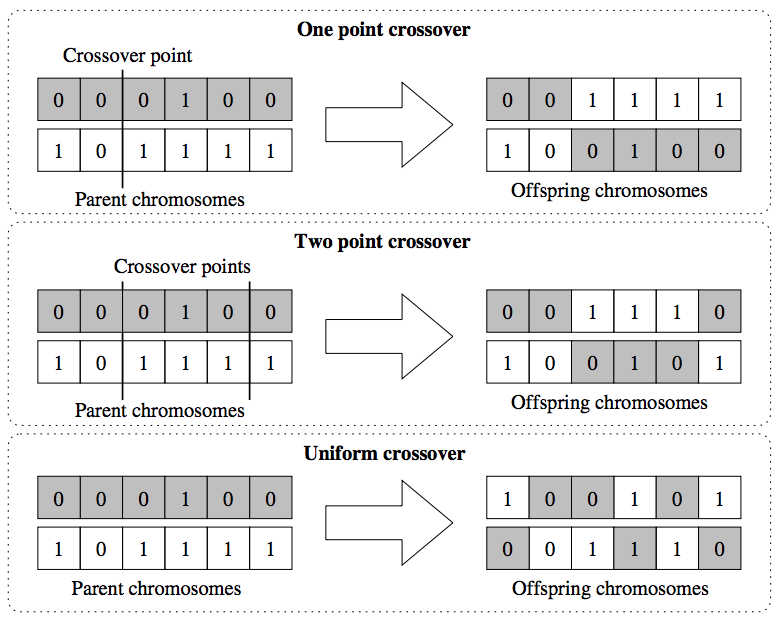
\includegraphics[scale=.8]{crossover.png}
  \caption{Crossover methods \cite{genetic}.}
  \label{fig:crossover}
\end{figure}

\subsection{Mutation}

Mutation randomly modifies a single candidate solution according to some
mutation probability. Essentially, this can be viewed as performing a random
walk in the vicinity of the individual chromosome solution.

\subsection{Replacement}

The offspring population replaces the original parent population. The offspring
population can replace \textit{all} of the parent population, or we can use
steady-state replacement to only replace \textit{n} new offspring.

\section{Snake Project} \label{section_snake}

We decided to apply the strategies of neural networks and genetic algorithms in
order to train an AI to play a game of snake. This sample implementation
provides a good testing ground for utilizing these strategies. The search space
for an AI to play snake is sufficiently large, that it is possible to see
improvements in the performance of the AI, but it is small enough that those
improvements do not take long.
% ARDEN

\subsection{Game Set-Up and Rules}

The first step of the process was to construct the game itself. The game
itself is very simple. A player controls a snake on a grid. The snake is
trying to eat food (an apple), and every time the snake eats a piece of food,
it grows in length by one. If the snake runs into the walls or itself, it dies.

We decided to split the game into four main functions.
\begin{enumerate}
  \item \textit{Initialize:} This function initializes the game state. This
    includes the position of the apple, the position of the snake, and the size
    of the grid. For most of our testing we defaulted to a grid of size 20.
  \item \textit{Get Move:} This function provides provides some interface with
    the current game state, and retrieves a direction to move in. This
    interface can either be a user input, or it could be some AI process.
  \item \textit{Update:} This function updates the game state provided with
    the direction to move in. This function moves the snake, and if it eats an
    apple, it extends the snake by one, and spawns a new apple on the grid.
  \item \textit{Valid:} This function checks if the current game state is
    valid. This is where we test to see if the snake has run into itself, or a
    wall.
\end{enumerate}

The basic structure of the snake program is to execute function 1 once, and
then while the game state is valid execute functions 2-3. The final part of the
game is the scoring system. Each update without dying increases the score by
1, and each apple eaten increases the score by 1000.

\begin{figure}[htpb]
  \begin{center}
    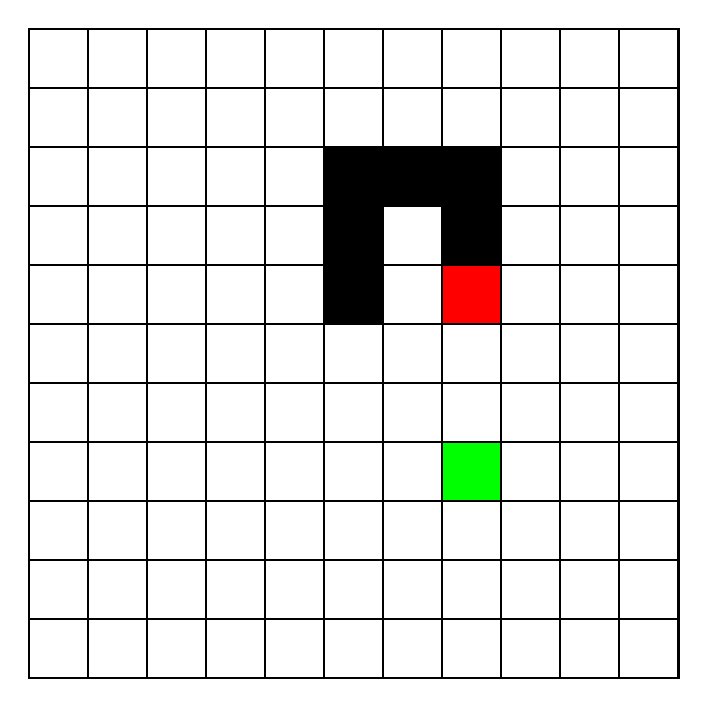
\begin{tikzpicture}[scale=0.75, transform shape,
      box/.style={rectangle,draw=black,thick,minimum size=1cm}]
      \foreach \x in {0,...,10}{
        \foreach \y in {0,...,10}{
          \node[box] at (\x,\y){};
        }
      }
      \node[box,fill=green] at (7,3){};
      \node[box,fill=black] at (5,6){};
      \node[box,fill=black] at (5,7){};
      \node[box,fill=black] at (5,8){};
      \node[box,fill=black] at (6,8){};
      \node[box,fill=black] at (7,8){};
      \node[box,fill=black] at (7,7){};
      \node[box,fill=red] at (7,6){};
    \end{tikzpicture}
  \end{center}
  \caption{Example game state for a snake game, here black denotes the snake
  body, green denotes the apple, and red denotes the snake head.}
  \label{fig:snake_game}
\end{figure}


Using this basic structure of the snake game, we determine that the
optimization problem at hand is to maximize the score of the game. Now we
construct the architecture of a neural network and genetic algorithm to solve
this optimization problem.

\subsection{Neural Network Structure}

Since any neural network requires a specific number of input, we decided on
utilizes rays. For each of the four directions from the snake, we cast a ray.
The ray will tell the neural network how far away something is in that
direction. For this we case three different rays in each direction.
\begin{enumerate}
  \item Apple Ray. Tells the network how far away the apple is in that
    direction, if at all.
  \item Snake Ray. Tells the network how far away the snake body is in that
    direction, if at all.
  \item Wall Ray Tells the network how far away the wall is in that direction.
\end{enumerate}
The casting of these rays can be seen in figures \ref{fig:snake_rays}.

\begin{figure}[htpb]
  \begin{center}
    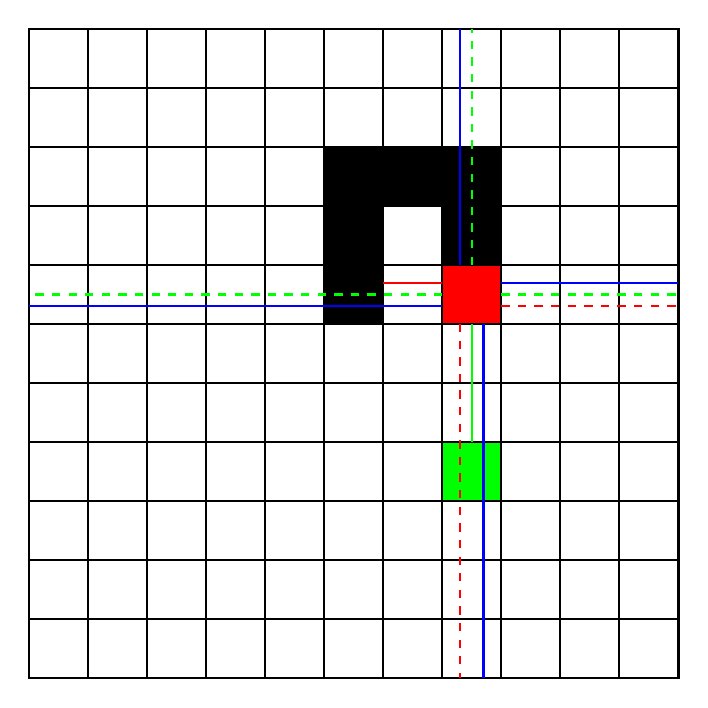
\begin{tikzpicture}[scale=0.75, transform shape,
      box/.style={rectangle,draw=black,thick,minimum size=1cm}]
      \foreach \x in {0,...,10}{
        \foreach \y in {0,...,10}{
          \node[box] at (\x,\y){};
        }
      }
      \node[box,fill=green] at (7,3){};
      \node[box,fill=black] at (5,6){};
      \node[box,fill=black] at (5,7){};
      \node[box,fill=black] at (5,8){};
      \node[box,fill=black] at (6,8){};
      \node[box,fill=black] at (7,8){};
      \node[box,fill=black] at (7,7){};
      \node[box,fill=red] at (7,6){};

      \draw[thick,color=green] (7,5.5) -- (7,3.5);
      \draw[thick,color=green,dashed] (7.5,6) -- (10.5,6);
      \draw[thick,color=green,dashed] (6.5,6) -- (-0.5,6);
      \draw[thick,color=green,dashed] (7,6.5) -- (7,10.5);

      \draw[thick,color=blue,] (7.2,5.5) -- (7.2,-0.5);
      \draw[thick,color=blue,] (7.5,6.2) -- (10.5,6.2);
      \draw[thick,color=blue,] (6.5,5.8) -- (-0.5,5.8);
      \draw[thick,color=blue,] (6.8,6.5) -- (6.8,10.5);

      \draw[thick,color=red,dashed] (6.8,5.5) -- (6.8,-0.5);
      \draw[thick,color=red,dashed] (7.5,5.8) -- (10.5,5.8);
      \draw[thick,color=red,] (6.5,6.2) -- (5.5,6.2);
      \draw[thick,color=red,] (7.2,6.5) -- (7.2,6.5);

    \end{tikzpicture}
  \end{center}
  \caption{Rays cast from the snake head. Green rays are the apple rays, red
    rays are the snake rays, and blue rays are the wall rays. If a ray is dashed,
  then it did not hit anything.}
  \label{fig:snake_rays}
\end{figure}

Once each ray has been cast, we pass the reciprocal of the distance to the
neural network. For example the down apple ray in figure \ref{fig:snake_rays},
would have a distance of $2$ since it travels two spaces before hitting the
apple. Thus the network would get a value of $\frac{1}{2}$. This is done so
that closer values are larger, and thus can easily be viewed as more important.

We also know that the output of the snake must be one of four values; Up, Down,
Left, or Right. Using this we constructed a neural network with $12$ input
neurons and $4$ output neurons. Most of the tests that we made were done
without any hidden layers, but it is also possible to insert hidden layers as
desired. The architecture of the network is demonstrated in figure
\ref{fig:snake_0layer}.

\begin{figure}[htpb]
  \begin{center}
    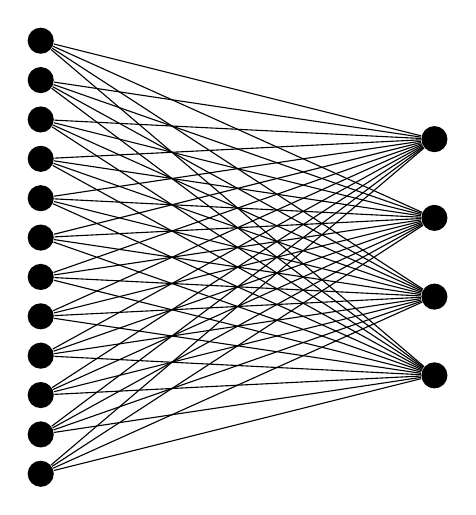
\begin{tikzpicture}[scale=1, transform shape]
      \node[circle,fill=black] (d00) at (0,-2.75) {};
      \node[circle,fill=black] (d01) at (0,-2.25) {};
      \node[circle,fill=black] (d02) at (0,-1.75) {};
      \node[circle,fill=black] (d03) at (0,-1.25) {};
      \node[circle,fill=black] (d04) at (0,-0.75) {};
      \node[circle,fill=black] (d05) at (0,-0.25) {};
      \node[circle,fill=black] (d06) at (0,0.25) {};
      \node[circle,fill=black] (d07) at (0,0.75) {};
      \node[circle,fill=black] (d08) at (0,1.25) {};
      \node[circle,fill=black] (d09) at (0,1.75) {};
      \node[circle,fill=black] (d010) at (0,2.25) {};
      \node[circle,fill=black] (d011) at (0,2.75) {};
      \node[circle,fill=black] (d10) at (5,-1.5) {};
      \draw (d00) -- (d10);
      \draw (d01) -- (d10);
      \draw (d02) -- (d10);
      \draw (d03) -- (d10);
      \draw (d04) -- (d10);
      \draw (d05) -- (d10);
      \draw (d06) -- (d10);
      \draw (d07) -- (d10);
      \draw (d08) -- (d10);
      \draw (d09) -- (d10);
      \draw (d010) -- (d10);
      \draw (d011) -- (d10);
      \node[circle,fill=black] (d11) at (5,-0.5) {};
      \draw (d00) -- (d11);
      \draw (d01) -- (d11);
      \draw (d02) -- (d11);
      \draw (d03) -- (d11);
      \draw (d04) -- (d11);
      \draw (d05) -- (d11);
      \draw (d06) -- (d11);
      \draw (d07) -- (d11);
      \draw (d08) -- (d11);
      \draw (d09) -- (d11);
      \draw (d010) -- (d11);
      \draw (d011) -- (d11);
      \node[circle,fill=black] (d12) at (5,0.5) {};
      \draw (d00) -- (d12);
      \draw (d01) -- (d12);
      \draw (d02) -- (d12);
      \draw (d03) -- (d12);
      \draw (d04) -- (d12);
      \draw (d05) -- (d12);
      \draw (d06) -- (d12);
      \draw (d07) -- (d12);
      \draw (d08) -- (d12);
      \draw (d09) -- (d12);
      \draw (d010) -- (d12);
      \draw (d011) -- (d12);
      \node[circle,fill=black] (d13) at (5,1.5) {};
      \draw (d00) -- (d13);
      \draw (d01) -- (d13);
      \draw (d02) -- (d13);
      \draw (d03) -- (d13);
      \draw (d04) -- (d13);
      \draw (d05) -- (d13);
      \draw (d06) -- (d13);
      \draw (d07) -- (d13);
      \draw (d08) -- (d13);
      \draw (d09) -- (d13);
      \draw (d010) -- (d13);
      \draw (d011) -- (d13);
    \end{tikzpicture}
  \end{center}
  \caption{Architecture of the snake AI neural network.}
  \label{fig:snake_0layer}
\end{figure}

Using this network architecture, there will be $48$ weights in the weight
matrix, and $4$ bias values in the bias vector. This means that there will be a
total of $52$ values that must be optimized.


\subsection{Training Network with Genetic Algorithm}

To optimize weights of a neural network, one must have training data, and the
answer key to that data. For situations like a game of snake. It is impossible
to know which direction it should go given every game state, so we are unable
to optimize a neural network in the classical method. This is why we implement
a genetic algorithm to optimize the neural network.

We construct a population of chromosomes, where each chromosomes has 52 genes.
We define a method for the conversion from the list of genes in the chromosome
to a neural network. The process is outlined below.

\begin{align*}
  \text{Chromo}=\left[x_1,\ldots,x_{52}\right]\implies
  W=\begin{bmatrix}
    x_1 & x_2 & \ldots & x_{12}\\
    x_{13} & x_{14} & \ldots & x_{24}\\
    x_{25} & x_{26} & \ldots & x_{36}\\
    x_{37} & x_{38} & \ldots & x_{48}\\
    \end{bmatrix},\quad B=\begin{bmatrix}
    x_{49} \\ x_{50} \\ x_{51} \\ x_{52}
  \end{bmatrix}
\end{align*}

For the evaluation stage of the genetic algorithm, each chromosome is converted
into a neural network, and it the plays the game of snake. The score returned
from that game is the fitness of the chromosome. Since the game has some
randomness in the generation of the apples. We evaluate each chromosome $5$
times, and average the scores to be the fitness. Then the rest of the genetic
algorithm proceeds as nominal, selecting the best chromosomes of the
population. After 20-50 generations, the network has usually made considerable
progress, and the learning curve has begun to plateau.

In the future it would be beneficial to experiment with additional layers, and
how having more layers of different sizes would effect the fitness of the
neural networks produced by the genetic algorithm.

\nocite{*}
\bibliographystyle{alpha}
\bibliography{main}

\end{document}
